\newcommand{\RNum}[1]{\uppercase\expandafter{\romannumeral #1\relax}}

\section{Study overview}
Studie \RNum{1} var å teste om kontekstuell interference kan bidra til å forbedre oppgavene utøverne blir satt til å løse. 

Studie \RNum{2} var å teste om reinforcement learning er en bedre læringsstrategi for å hjelpe utøvere til å ta gode strategivalg sammenlignet med tradisjonell coaching instruksjon (supervised learning). For å teste dette designet vi en læringsintervensjon som gikk over tre dager. I læringsintervensjonen brukte vi et between-subjects design og multi-armed bandit.  Studie \RNum{2} besvarte hvilke av disse strategiene som utøverne presterte best med. 


\begin{figure}[H]
\centering
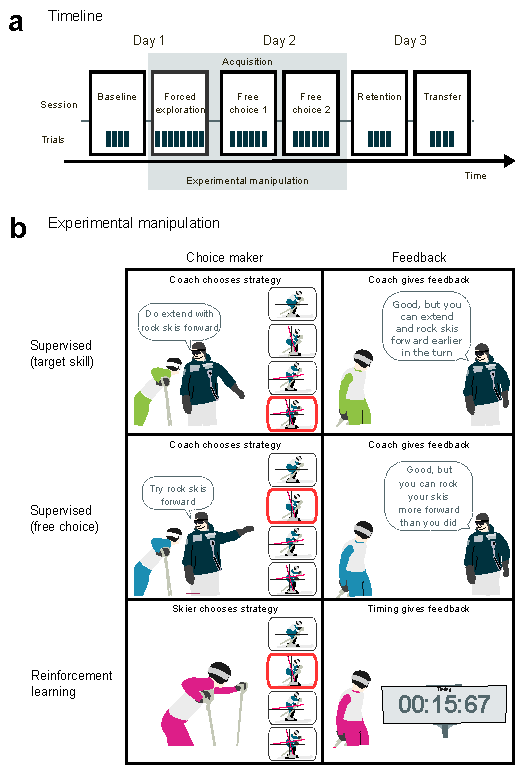
\includegraphics{figure_method_experiment.pdf}
\caption{Acceleration in the local positioning system section.\textbf{a.} Estimated acceleration during baseline and retention for the local positioning section. \textbf{b}. Expected mean difference between baseline and retention in the local positioning section.\textbf{c.} Estimated total gate-to-gate acceleration during baseline and retention in the local positioning section. \textbf{d}. Expected mean difference between baseline and retention in the local positioning section. The black lines denote the expected mean or differences in mean, with the shaded area representing their 95\% credible interval (CI). Each gray point or line represents one run trial by a skier}\label{fig: acc}
\end{figure}


\section{Setup}
All studies were conducted in the indoor ski hall, SNØ, located in Oslo, Norway (\url{https://snooslo.no/}). In this ski hall, we used the upper part of the race hill, which is a long flat section with two small rollers. The snow of this flat section was watered before testing each group of skiers to ensure uniform and fair conditions for all skiers. 

In study \RNum{1}, we set up three slalom courses to test the contextual interference effect. These courses required skiers to execute pumping movements with different timings and amplitudes for effective performance. All three courses had a vertical gate distance of 10 meters due to space constraints, forcing parallel setup. However, the courses had varying offsets: 1.2 meters for Course A, 1.7 meters for Course B, and 2.2 meters for Course C. These specific gate offsets were chosen to create diverse pumping demands without making it impossible to pump. Fig. 

In study 2, we set up two slalom courses to test. The main slalom course was used in all sessions except the transfer test and featured a 10-meter distance and a 1.9-meter offset. The transfer test assessed skiers' ability to transfer learning to a more realistic alpine race course. This test course included a progression in gate offset: five gates at 2.2 meters, seven gates at 1.7 meters, and seven gates at 1.2 meters. 

In both studies, we used stubbies (short gates) instead of long gates to minimize energy dissipation upon hitting the gate\cite{minetti_biomechanics_2018}. Using stubbies allowed skiers to focus better on skill execution of the strategy without the distraction of clearing the gate, which could hinder learning. In addition, this approach minimized hole creation that occurs when a long gate is forcefully slammed into the ground. 

We adopted the same standardized start procedure in both studies. The involved setting the start gate 20 meters before the first gate. Here, skiers were instructed to place their toe bindings behind the starting gate. Upon receiving the clearance signal, skiers were to place their skis parallel, lift the poles from the ground, and glide out of the start gate without using poling or skating to generate propulsion. Timing was recorded using a wireless photocell timing system (HC Timing wiNode and wiTimer; Oslo, Norway), starting when the skier crossed the first photocell pair situated 10 meters below the starting gate. (See https://osf.io/9numq for a supplementary video illustrating the starting procedure and setup).


\subsection{Participants}
Conducting studies on skilled alpine skiers presents several recruitment challenges. First, the population of skilled alpine skiers is relatively small and geographically dispersed across the country, which limits the number of participants available for testing. Additionally, these skiers must be willing to participate in the project. For coaches and skiers at this level to show this willingness, they must be convinced that the intervention will benefit the skiers' development, as it typically replaces the skiers' regular training due to their already high training volumes. Another limitation is the narrow time window for testing, typically in the spring and summer. This period is also popular for many ski teams to train indoors, leading to high demand for training lanes. Therefore, effective collaboration with the ski hall is crucial to gain permission to conduct research despite the high demand and to ensure the necessary support for the study. However, the ski hall can accommodate such studies only during a limited time of the year, further restricting the intervention period. These combined factors make it difficult to recruit a large number of participants.

Due to these resource constraints, our sample size approach in both studies was to recruit as many skiers as possible during the available testing window. To ensure that the skiers could handle the specific icy snow conditions prepared in the ski hall, we recruited skiers aged 15 years or older. Although some younger skiers participated in Study 1, they possessed the necessary skill level for the conditions. Beyond these criteria, we deliberately opted to recruit skiers with diverse skill levels to enhance the generalizability of our findings, despite not explicitly stating this in Study 1. In Study 1, we were uncertain about the expected effect sizes and our smallest effect size of interest, leaving our smallest effect size of interest unspecified. However, we learned much from this study. In Study 2, we set our smallest effect size of interest at a 0.3 second difference between groups. This benchmark was based on our knowledge of alpine skiing and discussions with coaches. However, it was intended for a 50-meter longer course and more training sessions than we ultimately used due to practical considerations. For Study 2, we set the minimum sample size to 80 skiers, which we deemed appropriate for this context. Prior to data collection, we conducted power simulations for sample sizes of 80, 100, and 120 skiers. These simulations revealed powers of 0.60, 0.75, and 0.80, respectively, for the smallest effect size of interest (0.3 seconds difference between groups) (\url{https://osf.io/c4t28}). 


\section{Design and procedure}

\subsection{Study 1}
In Study 1, we employed a between-subjects design and allocated skiers to either a blocked or interleaved learning group. The experiment began with a baseline test consisting of nine trials (three trials on each of courses A, B, and C), where skiers skied as quickly as possible without receiving time feedback. The trials in these courses were distributed randomly to each skier under the condition that the skier did not perform two consecutive runs on the same course. In addition, the skiers performed a straight gliding task on a dedicated lane before, midway (randomly assigned), and after the nine trials.

After the baseline test, we used a randomized-blocked design to allocate skiers into either the blocked or interleaved learning group based on their baseline test times. Specifically, we extracted each skier's best run from the baseline on each course and divided it by the average of the straight gliding runs from the baseline. Skiers were then ranked from fastest to slowest and paired in ascending order, and each consecutive pair was randomly assigned to either the interleaved or blocked group.

Immediately after the baseline test on day one, skiers attended a workshop where we explained the mechanical principles of the pumping technique and presented quantitative evidence supporting this strategy. Skiers then completed three training sessions over three days, with each session including 15 runs: 12 runs on the three courses and three straight-gliding runs. The interleaved group skied all three courses each day in a randomized interleaved order, ensuring no more than two consecutive runs on the same course. The blocked group performed all their runs on one course (A, B, or C) per day, with the course order counterbalanced across participants. 

Three days (72 hours) after the last training session, the skiers returned for a retention test, consisting of 12 runs (three runs on each of the three slalom courses and three straight-gliding runs). The order of the runs in the courses was scheduled in a semirandom order, with the condition that no more than two consecutive runs could be performed in the same course. As in the baseline test, the skiers performed a straight gliding task on a dedicated lane before, midway (randomly assigned), and after the nine trials. The skiers were instructed to ski as fast as possible but did not receive any performance feedback during the posttest. This design allowed us to compare the effects of blocked versus interleaved practices on the learning and performance of the pumping strategy. 


 \subsection{Study 2}
In study 2, brukte vi et between-subjects design og framet oppgaven om å velge gode strategier som et multi-armed bandit problem \cite{sutton_reinforcement_2018} (see methodeseksjonen i paper 3 for en beskrivelse av dette problemet). I denne studien var valgmulighetene (eller bandits) som utøverne måtte lære handlingsverdien og velge for å kjøre raskest mulig på ski de fire tekniske strategien vi har utbrodert i seksjon \ref{introduction: strategies}. 

Læringseksperimentet begynte med en baseline som bestod av fire runder i slalåmløypen (main course in fig), pluss en straightgliding runde der utøverne kjørte ned løypeseksjonen i en egen dedikert bane for dette. Før utøverne gjennomførte disse fire rundene og straight glidingen gjennomførte de to oppvarmingsrunde: en gjennomført som frikjøring og som gjennomført som oppvarming i løypen, der de fikk instruksjoner og tilbakemelding på utførelsen av startprosedyren. 

Etter dette delte allokerte vi utøverne i tre læringsgrupper








































